

\documentclass[a4paper, 12pt]{article}
\usepackage[a4paper,margin=0.9in]{geometry}
\usepackage[utf8]{inputenc}
\usepackage[frenchb]{babel}
\usepackage{indentfirst}
\usepackage{dirtree}
\usepackage{tikz}
\usepackage{amsmath}
\usepackage{framed}
\usepackage{parskip}
\usepackage{calc}
\usepackage{subfig}
\usepackage{hyperref}
\usepackage[toc,page]{appendix}
\usepackage{parskip}
\usepackage{listings}
\usepackage{color}
\usepackage{verbatim}
\usepackage{graphicx}
\usetikzlibrary{shapes,arrows}
\usetikzlibrary{trees}

\setlength{\parskip}{12pt}

\title{Réseau Sémantique à partir d'un dictionnaire}
\author{Bawden Rachel, Brogniez Caroline et Parslow Nicholas}
\date{}

\begin{document}
\tikzstyle{every node}=[thick,anchor=west]
\tikzstyle{selected}=[draw=red,fill=red!30]

\tikzstyle{decision} = [diamond, draw, fill=blue!20, 
    text width=4.5em, text badly centered, node distance=3cm, inner sep=0pt]
\tikzstyle{block} = [rectangle, draw, fill=blue!20, 
    text width=5em, text centered, rounded corners, minimum height=4em]
\tikzstyle{line} = [draw, -latex']
\tikzstyle{cloud} = [draw, ellipse,fill=red!20, node distance=3cm,
    minimum height=2em]

\maketitle

\section{Introduction}


\section{La Conception du Graphe}

La construction d'un réseau sémantique à partir d'un dictionnaire est possible grâce à la structure des dictionnaires qui permet de faire ressortir des liens sémantiques. La structure en sens, sous-sens, définitions, et exemples, parmi d'autres informations, mais aussi la structure interne des définitions contient une régularité qu'il est important d'exploiter au maximum. Nous tenons donc à conserver le plus possible cette structure dans la transformation de dictionnaire en graphe. 
Un graphe est défini formellement comme un ensemble de sommets et un ensemble d'arcs qui relient une paire de sommets.

\[
G = <S, A>
\]

Pour représenter un dictionnaire par un graphe, nous considérons que les sommets peuvent être les mots individuels du dictionnaire ou même les niveaux intermédiaires de la structure tels que 'exemple', 'définition', 'synonyme', 'antonyme' etc. Les arcs sont alors les liens qui lient les différents éléments d'une entrée de dictionnaire et permettraient de trouver un lien entre un lexème donné et la manière dont il est décrit dans son entrée du dictionnaire.

\subsection{Remarques sur le vocabulaire}
Nous appelons 'mot' toute unité minimale du lexique. Un mot peut être soit fléchi, soit non-fléchi et par défaut nous faisons référence aux mots non-fléchis sous leur forme de dictionnaire. Par principe, nous restreignons le réseau aux lemmes, mais il est possible qu'il y apparaît des formes fléchies en cas de non-identification du lemme.

Par 'entrée' de dictionnaire nous faisons référence à un groupe d'informations (catégories syntaxiques, sens, définitions, exemples etc.) associées à un mot donné. Par conséquent, le terme 'entrée' peut aussi être utilisé pour dénoter le mot lui-même, et par extension les informations contenues pour ce mot donné.

La relation sémantique de synonymie est définie entre deux termes de la même catégorie de discours qui ont le même sens et qui peuvent donc être substitués l'un pour l'autre sans modifier le sens de la phrase. Cette définition pose évidemment des problèmes, surtout à cause du fait qu'il est toujours possible de trouver une différence de sens ou d'usage entre deux mots malgré le fait qu'ils soient habituellement classés en synonymes. Il est parfois souhaitable de parler de proche-synonymes au lieu de synonymes tout court. Néanmois, nous préférons utiliser le terme 'synonyme' pour parler de ces cas, sans postuler de théorie sur les frontières de la synonymie. Par la suite, la synonymie sera définie en termes de relations attestées dans des ressources externes et nous nous reportons à ces références pour établir si deux mots sont en relation de synonymie ou pas.

De même pour les relations d'antonymie, d'hyperonymie et d'hyponymie. L'antonymie est définie comme la relation entre deux mots à sens opposé. L'hyperonymie entre un mot dont l'extension contient l'extension d'un autre mot (par exemple, 'véhicule' est l'hypernym de 'voiture'). l'hyponymie est la relation inverse d'hyperonymie, entre un mot dont l'extension est incluse dans l'extension d'un autre (pour reprendre le même exemple, 'voiture' est un hyponyme de 'véhicule').

[AUTRES DEFINITIIONS...]

\section{La structure des dictionnaires utilisés}

Les deux ressources qui seront utilisées sont le Wiktionnaire français en format XML du CLLE-ERSS dans le cadre du projet WiktionaryX \hyperref[bib:wikixml]{[~\ref*{bib:wikixml}]} et le Littré , qui est aussi disponible en format XML \hyperref[bib:littrexml]{[~\ref*{bib:littrexml}]}.

Les informations contenues dans les deux dictionnaires sont similaires. Chaque dictionnaire est organisé en entrées, et chaque entrée contient plusieurs définitions, des exemples, des synonymes et des informations grammaticales. Le wiktionnaire contient en plus d'autres relations sémantiques telles que l'antonymie, l'hyperonymie et l’hyponymie.

\subsection{Statistiques}

NOMBRE d'ENTREES
NOMBRE DE CATS SYNT DIFF
NOMBRE DE MOT-FORMES DIFF

\section{Pré-traitement}

Dans le but de pouvoir procéder à un traitement homogène des deux dictionnaires, une normalisation des deux formats était nécessaire. Ce pré-traitement a permis à la fois de supprimer certaines informations qui n'étaient pas utilisée par la suite et de convertir les balises et leur contenu en un format plus convenable pour notre traitement. Nous réunissons les deux structures dans un seul type de fichier XML avec les balises suivantes:

    \begin{itemize}
        \item[$\circ$] entry : un mot du dictionnaire (lexème)
        \item[$\circ$] pos : la catégorie syntaxique (il peut y en avoir plusieurs par lexème)
        \item[$\circ$] sense : le niveau hiérarchique représentant plusieurs sens d'un même mot
        \item[$\circ$] subsense : le niveau hiérarchique représentant plusieurs sous-sens d'un même sens global
        \item[$\circ$] def-text : le texte d'une défintion
        \item[$\circ$] semantic : l'emploi sémantique d'un mot (figuratif, absolu etc.)
        \item[$\circ$] register : le registre du mot (familier, vulgaire, soutenu etc.)
        \item[$\circ$] domain : le domaine sémantique du mot (géographie, biologie, culinaire etc.)
        \item[$\circ$] refs : des références vers d'autres entrées lexicales
        \item[$\circ$] examples : des phrases exemples contenant le mot de l'entrée lexicale
        \item[$\circ$] synonyms : synonymes de du mot de l'entrée
        \item[$\circ$] antonyms : antonymes de du mot de l'entrée
        \item[$\circ$] hyperonyms : hyperymes de du mot de l'entrée
        \item[$\circ$] hyponyms : hyponymes de du mot de l'entrée
    \end{itemize}
\bigskip

La DTD des fichiers XML normalisés se trouve dans l'appendice \hyperref[App:dtddico]{~\ref*{App:dtddico}}, avec les scripts de normalisation\hyperref[App:normlittre]{~\ref*{App:normlittre}} et \hyperref[App:normwiki]{~\ref*{App:normwiki}}.
\hyperref[fig:XMLhierarchy]{Figure~\ref*{fig:XMLhierarchy}}  illustre l'hiérarchie des balises, qui correspond aussi à la structure théorique du réseau.

\begin{figure}[!ht]
\centering
\def\svgwidth{\columnwidth}
%\input{schema.pdf_tex}
\input{filler.pdf_tex}
\caption{L'hiérarchie des entrées définie pour les dictionnaires en XML}
\label{fig:XMLhierarchy}
\end{figure}


De légères différences existent entre les structures des deux dictionnaires. Tandis que la plupart des informations du Wiktionnaire sont localisées au niveau du 'sense', la plupart des informations du Littré sont localisées au niveau du 'subsense', ce qui ne pose aucun problème pour la construction des deux réseaux.
\newline
\newline
En plus de la restructuration des fichiers XML, les dictionnaires ont été nettoyés pour convenir à nos besoins. Certaines balises contiennent trop d'informations ou des informations non-pertinentes. Par exemple, les balises des commentaires pour le Littré ne contiennent pas de contenu exploitable et les citations des textes anciens des mots vieillis qui risquent d'ajouter du bruit dans le réseau résultant. Les entrées sont ainsi réduites au schéma ci-dessus (\hyperref[fig:XMLhierarchy]{Figure~\ref*{fig:XMLhierarchy}}). Le Littré en particulier nécessite une étape importante de nettoyage, puisque des erreurs existent dans le balisage des données et un manque d'homogénéité dans la structuration des entrées risque de perturber la manière dont laquelle les relations sont établies entre les éléments qu'elles contiennent. Les catégories syntaxiques utilisées ne sont pas d'une liste énumérable et contiennent des descriptions plutôt littéraires. Cette étape de normalisation consistait aussi à traduire ces catégories syntaxiques en une liste plus formelle et identifiable.

Les définitions, exemples et autres informations dans les entrées étaient ensuite taggés et lemmatisés en utilisant l'outil MElt (\hyperref[bib:melt]{[~\ref*{bib:melt}]}). Cette étape est importante pour pouvoir relier les mots fléchis des définitions avec leurs lemmes tels qu'ils apparaissent dans les entrées et pour savoir de quelle catégorie syntaxique il s'agit. Le script XXX qui sert à tagger et lemmatiser les documents se trouvent dans l'annexe \hyperref[App:tag]{[~\ref*{App:tag}]}.

\section{La représentation en graphe}

Les fichiers XML sont facilement transférables en représentation en graphe, puisqu'ils continennent une hiérarchie d'entrées. En principe chaque niveau de l'hiérarchie est représenté par un nœud différent avec des arcs qui lie chaque nœud à ses fils dans l'hiérarchie, comme dans \hyperref[fig:XMLhierarchy]{Figure~\ref*{fig:XMLhierarchy}}. Cette représentation a l'avantage de préserver la structure hiérarchique d'origine.

En plus des arêtes descendantes qui existent dans le schéma \hyperref[fig:XMLhierarchy]{Figure~\ref*{fig:XMLhierarchy}}, nous établissons des arêtes montantes, afin de retrouver facilement la relation entre un mot qui apparaît dans une entrée et le lexème de l'entrée. Les poids sur ces arêtes ne sont pas les mêmes que les arêtes descendantes afin de retrouver une différence dans ces relations.


\section{La pondération des relations}

Pour injecter plus de sophistication dans le réseau, la distance entre deux mots ne se limite pas au nombre d'arêtes dans le chemin. Les arêtes sont pondérées selon le type de nœud sortant et entrant afin de distinguer entre les relations différentes qui peuvent exister à différents endroits de l'entrée. Contrairement aux réseaux sémantiques plus sophistiqués tels que WordNet\hyperref[bib:wordnet]{[~\ref*{bib:wordnet}]}, qui encodent des relations typées spécifiques, notre réseau se base sur un principe plus simple de pondération, avec des valeurs réelles assignées par rapport à l'emplacement des mots dans l'entrée du dictionnaire.

Les poids des arêtes font partie des paramètres du réseau et sont conservés dans un fichier de configuration externe (weight.config), les valeurs étant choisies pour optimiser le réseau pour une tâche particulière. L'optimisation sera discutée dans la partie [XXX]. Il existe un total de 42 liens différent [CHECK] avec un poids différent entre zéro et infinité, un lien de 0 étant un lien non-existant dans le graphe.

Ci-dessus un extrait de ce fichier, qui se trouve dans l'annexe [REF] :

\begin{framed}
entry2pos = 0.01\newline
pos2entry = 0.01\newline
pos2sense = 0.01\newline
sense2pos = 0.01\newline
pos2syn = 0.01\newline
syn2pos = 0.01\newline
...\newline
sense2subsense = 0.001\newline
subsense2sense = 0.001\newline
subsense2deftext = 0.00001\newline
deftext2subsense = 0.00001\newline
subsense2semantic = 0\newline
\end{framed}

En plus de ces paramètres basés uniquement sur la structure des entrées, d'autres paramètres sont utilisés pour faire ressortir des informations lexicales en plus de ces relations déjà trouvées. Ces paramètres se trouvent dans un deuxième fichier de configuration, qui peut être modifié de la même façon que le fichier de poids. La différence est que l'utilisateur peut spécifier le type d'opération à effectuer sur le poids d'origine. Chaque paramètre est écrit sur une seule ligne avec l'étape de la création du graphe à laquelle le paramètre sera implémenté, ainsi que d'autres options utilisées pour spécifier comment le paramètre peut être utilisé.

Etant donné un mot x et un mot y, où x est le mot d'entrée et y le mot de sa définition, le poids d'origine serait le poids spécifié entre un mot d'entrée et sa définition (c'est-à-dire entry2pos + pos2sense + sense2subsense + subsense2deftext). Ensuite ce poids peut être transformé de plusieurs façons:


\subsection{En fonction des propriétés catégorielles}
Pendant l'étape de préparation du graphe, avant la création de la matrice, les poids sont traffiqués en fonction des propriétés catégorielles pour donner plus ou moins de poids à certaines catégories. Les paramètres sont de la forme suivante :
    \begin{framed}
        POS\_de\_y, POS\_de\_x, fichiers\_contextes, opération\_math, valeur
    \end{framed}

\subsubsection{Modification uniquement en fonction de la catégorie syntaxique du mot y.}
Ces paramètres servent à privilégier certaines catégories de mot par rapport à d'autres, en supposant que certaines catégories sont plus utiles pour établir des relations sémantiques.[XXX PARLER PLUS] Un paramètre est spécifié pour chaque catégorie syntaxique afin d'établir des modifications relatives entre catégories. Par exemple, pour la catégorie \lq{adjectif}\rq: \lq{prepare: Adj, None, None, +, 0.6}\rq signifie que 0.6 est ajouté à tout noeud qui va vers un mot de catégorie \lq{Adj}\rq.

\subsubsection{Modification en fonction de la catégorie syntaxique du mot x, du mot y et d'un fichier de contextes spécifiques.} 
Jusqu'à présent le poids des relations a été fondé uniquement sur l'emplacement des mots y dans l'entrée et de leurs catégories syntaxiques. Mais il est aussi important d'analyser la structure des informations à l'intérieur des définitions, puisque les définitions font preuve d'une régularité qui permet de donner plus de poids à certains mots. Sans faire une analyse syntaxique complète des définitions, nous visons à cibler certains mots qui apparaissent dans un certain contexte afin de renforcer la relation entre le mot de l'entrée et ces mots cibles. La forme du paramètre dans le fichier de configuration est la même que pour les paramètres précédents, sauf que la deuxième option \lq{POS\_de\_x}\rq est spécifiée, ainsi que le chemin vers le fichier de contextes légitimisants.
\newline\newline
Nous jugeons nécessaire de spécifier la catégorie syntaxique du mot x ainsi que la catégorie du mot y parce que la forme de la définition dépend en grande partie de la catégorie syntaxique du mot de l'entrée et la relation entre un mot x de catégorie 'nom' et un mot y de catégorie \lq{nom}\rq n'est pas la même relation que celle entre un mot x de catégorie \lq{nom}\rq et un mot y de catégorie \lq{verbe}\rq.
\newline\newline
Par exemple, pour un mot x de catégorie \lq{adverbe}\rq, il pourrait être pertinent de renforcer le lien entre x et y, si y est un adjectif qui apparaît dans le contexte \lq{d'une manière mot\_y}\rq.

\underline{Syntaxe}\newline
Nous définissons une syntaxe particulière pour représenter les contextes légitimisants. En général ce sont une séquence de mots précédant et/ou suivant le mot y en question, qui signale que ce mot doit être mis en valeur.\newline

\begin{itemize}
    \item{Les contextes précédents et suivants sont des séquences de mots. Ces séquences peuvent contenir soit des mots-formes, soit des lemmes, ce qui permet plus de flexibilité dans la rédaction des règles et de ne pas devoir expliciter toutes les combinaisons de formes fléchies possibles.}

    \item{\# représente la position du mot y, ce qui permet de spécifier le contexte précédent et le contexte suivant du mot.}

    \item{Les symboles \string^ et \$ représentent respectivement le début et la fin de la phrase}

    \item{Un chiffre indique le nombre maximum de mots qui peuvent apparaître à une position donnée, sans devoir spécifier la forme ou le lemme de ces mots. Notez que ces mots ne peuvent pas être un signe de ponctuation ou de la même catégorie syntaxique que le mot y. Ceci fait en sorte que ce soit le premier mot de la catégorie recherchée qui est renforcée par ce contexte.}

\end{itemize}

Par exemple, dans l'entrée du mot \lq{langoureusement}\rq, la définition \lq{d'une manière langoureuse}\rq et le contexte légitimisant \lq{de une manière \#}\rq permettrait de renforcer la relation entre \lq langoureusement\rq et \lq langoureux\rq, ce dernier apparaissant dans la position spécifiée par \#. Dans cet exemple, il n'y a pas de contexte suivant spécifié (puisqu'aucun mot ne suit le \#) et ceci est le cas dans la plupart des contextes, où le contexte précédent est le plus important. Pour simplifier les contextes, nous permettons de ne pas exprimer le \# et dans ce cas, la séquence de mots est considérée comme la séquence précédente du mot y. Pour reprendre l'exemple précédent, le contexte \lq{de une manière \#}\rq peut également être exprimé \lq{de une manière}\rq. Notons que si un contexte suivant est explicité, le \# est nécessaire.

Ci-dessous quelques exemples de contextes pour une paire de catégories pour les mots x et y:

\begin{table}[ht]
\centering
\begin{tabular}{|p{1cm}|p{1cm}|p{5.5cm}|p{8cm}|}
\hline
POS de x & POS de y & Contexte & Description\\[0.5ex]
\hline
Adj & Adj & . \# . & Un adjectif entre deux points \\
Nom & Nom & \string^ \# ,  & Un nom au début de la définition, suivi d'une virgule \\
Nom & Nom & synonyme de & Un nom qui suit la séquence \lq{synonyme de}\rq \\
Adj & Verbe & en parlant de une personne qui 3 & Un verbe qui suit la séquence \lq{en parlant de une personne qui}\rq avec un maximum de 3 mots intervenants qui ne sont pas de catégorie PONCT ou V \\
Adj & Nom & qui a des rapports avec 2 & Un nom qui suit la séquence \lq{qui a des rapports avec}\rq avec un maximum de 2 mots intervenants qui ne sont pas de catégorie PONCT ou N \\ [1ex]
\hline
\end{tabular}
\caption{Quelques exemples de contextes légitimisants}
\label{table:nonlin}
\end{table}


Les contextes ont été choisis en analysant les entrées de dictionnaire pour chaque type de catégorie syntaxique et en remarquant les régularités. Quelques contextes sont applicables pour un nombre de catégories différentes, par exemple \lq{synonyme de}\rq, \lq{hyperonyme de}\rq, et d'autres sont plus spécifiques aux contextes.

Chaque contexte est un tuple contenant une expression régulière pour le contexte précédent et une expression régulière pour le contexte suivant.

Les séquences sont transformées de la façon suivante:
\begin{itemize}
    \item{Toute la ligne est divisée en deux sur le symbole \#. S'il n'existe pas de symbole \#, toute la séquence est le contexte précédent est le contexte suivant est null.}
    \item{Pour chaque contexte (précédent et suivant), l'expression régulière est générée:}
    \begin{itemize}
        \item{tout caractère qui est un caractère spécial pour les expressions régulières doit être échappé (sauf \^ et \$ qui retiennent leur propriété de caractères spéciaux)}
        \item{tout mot est converti en une entité taggée et lemmatisée tel que le mot peut être considéré comme le mot-forme ou le lemme du mot.
Par exemple \lq{mot}\rq  est transformé en 
((mot/[\string^ /]+?/[\string^ /]+?)|([\string^ /]+?/[\string^ /]+?/mot)) }
    \end{itemize}
\end{itemize}

\underline{L'implémentation en Python}\newline
La correspondance entre les contextes d'un mot à l'intérieur d'une définition et les contextes légitimisant se fait par des expressions régulières, qui sont générées à partir des contextes des fichiers.

\section{La création du graphe}

\subsection{Choix de langage et de bibliothèques}
Nous implémentons le graphe en python, pour lequel il existe de nombreuses bibliothèques (Scipy, NumPy) efficaces qui permettent de manipuler un grand nombre de données numériques. Nous utilisons cElementTree pour traiter les fichiers XML et les SparseMatrices de NumPy pour représenter le graphe. Le réseau est alors une matrice NxN où N est le nombre de nœuds différents dans le graphe. Etant donné le grand nombre d'entrées dans les dictionnaires, il y a un avantage clair d'utiliser les matrices sparses, qui permettent de stocker plus efficacement un graphe qui contient de nombreux sommets et peu d'arêtes.

\subsection{Simplification de la structure}
En pratique, il est possible de surpasser d'un grand nombre de nœuds intermédiaires dans l'hiérarchie en attribuant une arête directe entre une paire de mots dont le poids serait l'addition de toutes les valeurs des liens qui constituent le chemin entre les deux mots. Le choix des sommets est un compromis entre mettre le plus d'informations possible dans le graphe et veiller à la non-explosion de la taille du graphe. Ceci n'est que possible parce que dans les tâches effectuées (détaillés dans la partie XXX), nous n'aurons jamais besoin d'extraire ces nœuds intermédiaires, même si nous souhaitons tenir compte de leur présence.

Ainsi, l'entrée dans \hyperref[fig:banane_full]{Figure~\ref*{fig:banane_full}} est simplifiée en l'entrée dans \hyperref[fig:banane_simple]{Figure~\ref*{fig:banane_simple}}:

\begin{figure}
\centering
\parbox{5cm}{
\def\svgscale{0.5}
%\input{entry_banane_full.pdf_tex}
\input{filler.pdf_tex}
\caption{First.}
\label{fig:banane_full}}
\qquad
\begin{minipage}{5cm}
\def\svgscale{0.5}
%\input{entry_banane_simple.pdf_tex}
\input{filler.pdf_tex}
\caption{Second.}
\label{fig:banane_simple}
\end{minipage}
\end{figure}

Notons que nous préservons deux niveaux d'hiérarchie pour le mot d'entrée : un contenant le mot seul et l'autre contenant aussi sa catégorie syntaxique. Ceci est un moyen d'assurer à ce que le mot soit trouvable dans le réseau sans devoir spécifier une catégorie syntaxique particulière, tout en permettant de faire la distinction entre plusieurs catégories syntaxiques pour un mot donné. Chaque mot taggé à l'intérieur d'une entrée est ainsi lié à une version non-taggée qui représente le niveau 'entry' de ce mot, même s'il n'existe pas comme entrée dans le dictionnaire de départ.

Le résultats est un graphe qui contient deux sortes de nœuds des mots non-taggés (correspondant au niveau entry' et des mots non-taggés (correspondant au niveau 'pos').

[IMAGE plein d'arêtes].

\subsection{La création du graphe}
Comme mentionné précedemment, le graphe lui-même est implementé en forme de matrice

\subsection{Wiktionnaire}


\section{Création du graphe}


\section{Synonymes}
\subsection{Programme}

\subsection{Evaluation}

\section{Désambiguation}
\subsection{Programme}

\subsection{Evaluation}


\section{Le Bras Droit du Cruciverbiste (i.e. La Résolution de Mots Croisés)}

La troisième tâche est la résolution d'indices de mots croisés. Le concept est simple et ressemblent aux tâches précédentes dans son exploitation du réseau sémantique. Tandis que le chercheur de synonymes calcule la distance entre des mots individuels et le désambiguïseur trouve la distance entre deux séquences de mots, le resolveur de mots-croisés cherche la distance entre une séquence de mots (l'indice) et un mot (le mot cible). Comme précédemment, le noyau du programme est donc une recherche de la matrice de relations pour trouver un certain nombre de mots candidats. Par contre, des étapes supplémentaires sont nécessaires pour faire en sorte que les mot cibles adhèrent à certaines contraintes imposées par le jeu.

Le principe des mots croisés est de remplir une grille de lettres en fonction d'indices, de longueur de mots cibles et de caractères qui ont déjà été devinés dans la grille. Notre application est un outil support qui permet de fournir des mots candidats au cruciverbiste\footnote{Un amateur de mots croisés}. A part ces deux contraintes, il est important que les mots candidats correspondent à la catégorie syntaxique indiquée par l'indice. Notons que pour l'instant l'application ne détecte que les mots des catégories \lq{nom}\rq, \lq{adj}\rq, \lq{adv}\rq{} et \lq{verbe}\rq, puisque les autres catégories ne sont pas présentes dans le réseau. Par exemple, pour une indice \lq{escroqués}\rq, les mots candidats doivent être des participes passés qui sont conjugués au masculin pluriel, et pour une indice \lq{a l'air chouette}\rq, les mots candidats doivent être des verbes conjugués au troisème personne singulier du présent indicatif\footnote{Les bonnes réponses sont \lq{eus}\rq{}  et \lq{ulule}\rq{} respectivement}.

Le processus suivi est donc séquentiel et peut être représenté par le schéma suivant:   

\begin{figure}[!ht]
\centering
\def\svgwidth{\columnwidth}
%\input{crossword_schema.pdf_tex}
\input{filler.pdf_tex}
\caption{Le schéma du traitement pour la résolution des indices de mots croisés}
\label{fig:schema_crosswords}
\end{figure}

\subsection{Les étapes de traitement}
\subsubsection{Etape 1 : Identification de la catégorie syntaxique du mot cible}
Les indices sont de petites séquences de mots qui sont très rarement des phrases complètent et bien formées. Elles correspondent souvent à un syntagme particulier et contiennent parfois des ambiguïtés de catégorie syntaxique. Il est aussi possible à cette étape d'identifier quelques marques de flexion qui peuvent indiquer la forme du mot cible. Le réseau sémantique ne contient a priori ques des lemmes et donc il est important de garder ces indices flexionnelles pour reconjuguer les mots candidats à l'étape 3 [REF].  

Un étiqueteur syntaxique automatique tel que MElt[\hyperref[bib:melt]{~\ref*{bib:melt}}] est peu adapté pour cette identification puisqu'il se base sur les probabilités pour renvoyer la séquence de tags la plus probable pour l'indice. Ceci signifie que le tag prédit peut ne pas correspondre à un des tags possibles pour un mot donné ou les ambiguïtés ne sont pas peut-être pas toutes reperées. De plus, de tels étiqueteurs sont dépendants de leurs données d'entraînement, et les indices des mots croisés sont d'une forme très différente des données du FTB sur lequel MElt a été entrainé. Nous choissisons donc de faire une analyse point à point des mots de l'indice afin de renvoyer toutes les possibilités catégorielles pour chaque mot. Le Lefff (Lexique des Formes Fléchies du Français)[\hyperref[bib:lefff]{~\ref*{bib:lefff}}] est utilisé pour retrouver toutes les catégories syntaxiques et marques flexionnelles de chaque mot. Cette méthode renvoie évidemment plus de catégories syntaxiques que souhaitées et crée de l'ambiguïté artificielle. Cependant, la précision des catégories renvoyées pour chaque mot est plus élevée et globalement le rappel est très élevé pour la séquence de mots. [EXPLAIN]

La catégorie cible peut être identifiée à partir de ces ensembles de catégories grâce à la régularité des formes des indices. Si une indice contient un seul mot, les catégories cibles sont celles du mot de l'indice. Sinon, la catégorie dépend en grande partie des premiers mots de l'indice. Par exemple, si une indice commence par un nom, ou une séquence \lq{det nom}\rq{} ou une séquence \lq{det adj nom}\rq{}, la catégorie cible, étant donné qu'il n'y a pas d'ambiguïté catégorielle serait, serait un nom. Dans certains cas, il est aussi possible d'identifier quel mot de l'indice indique la conjugaison du mot cible. Cette identification se fait à l'aide d'une mini-grammaire de seulement 14 règles, qui sont reproduites ci-dessous :

\begin{framed}
det nc -\textgreater 2, nc\newline
det adj nc -\textgreater 3, nc\newline
adj nc -\textgreater 2, nc\newline
nc -\textgreater 1, nc\newline
adj prep -\textgreater 1, adj\newline
adv v -\textgreater 2, v\newline
advm v -\textgreater 2, v\newline
advneg v -\textgreater 2, v\newline
advneg advneg v -\textgreater 3, v\newline
v -\textgreater 1, v\newline
clr v -\textgreater 2, v\newline
prel v -\textgreater 2, adj \newline
cln v -\textgreater 2, n\newline
prep nc -\textgreater ?, adj
\end{framed}

Chaque ligne représente une règle différente. A gauche de la flèche est la séquence de mots qui indiquent, au début d'une indice, une certaine catégorie syntaxique. A droite de la flèche est l'indice (à partir de 1) du mot de la partie gauche dont les informations grammaticales seront utilisés pour conjuguer les mots cibles, et ensuite est la catégorie syntaxique du mot cible. 

Le jeu d'étiquettes utilisées est celle du Lefff\footnote{Ce jeu a été réduit pour ne contenir que les noms, adjectifs, adverbes et verbes}, qui est utilisée pour retrouver les formes fléchies. Une même indice peut correspondre à plusieurs règles différentes si un mot donné est ambigu pour la catégorie syntaxique.

Les catégories syntaxiques sont retenues pour le parcours du réseau et les informations grammaticales pour retrouver les formes fléchies correspondant aux lemmes trouvés dans le réseau.

Une particularité des indices est que parfois elles peuvent contenir plusieurs parties, séparées d'une virgule et qui représentent plusieurs sous-indices à l'intérieur de l'indice. Par exemple, une indice peut avoir la forme \lq{habillée, fringuée}\rq{} et dans ce cas, il est souhaitable de séparer cette indice en \lq{habillée}\rq{} et \lq{fringuée}\rq{} afin d'avoir la meilleur chance de trouver la catégorie voulue. Idéalement, ces deux parties devraient aussi correspondre en termes de catégorie syntaxique, ce qui signifie qu'il faudrait en théorie ne garder que les catégories cibles qui correspondent aux deux parties de l'indice. Par contre, nous optons pour le choix de garder toutes les catégories potentielles à partir des deux parties de l'indice pour nous assurer de la couverture maximale. 

\subsubsection{Etape 2 : Recherche du graphe}

A partir des lemmes trouvés dans le Lefff pour chaque mot de l'indice, et à partir de formes fléchies si les mots ne s'y trouvent pas\footnote{Même si le réseau ne devraient pas contenir de formes fléchies, il est possible qu'il en contient à cause des erreurs de tagging, et donc nous exploitons cette faiblesse ici pour augmenter la chance de retrouver le plus de mots de l'indice possibles.}, un vecteur de mots avec leur distance est obtenu pour représenter toute l'indice. Ce vecteur contient la moyenne des vecteurs des vingt plus proches voisins obtenus pour chaque mot dans un parcours du réseau. Cette moyenne permet de calculer les mots les plus proches de l'indice en général. Les catégories de mots recherchés sont les catégories obtenues à partir des règles de la mini-grammaire. Dans le cas où aucun règle correspond à l'indice, notamment dans le cas où un des premiers mots de l'indice ne se trouve pas dans le lexique, les mots recherchés sont de n'importe quelle catégorie.

\subsubsection{Etape 3 : Conjugaison des lemmes obtenus}

Les résultats de la recherche du graphe sont des lemmes, qui sont à modifier pour correspondre à la forme du mot recherché. En utilisant l'ensemble de catégories et d'informations grammaticales obtenues lors de l'étape 1 [REF], cette étape cherche les formes fléchies correspondantes à chaque lemme et vérifie lesquelles correspondent aux informations grammaticales recherchées pour les mots candidats.

\subsubsection{Etape 4 : Filtrage selon les contraintes}

La dernière étape filtre les candidates conjugués afin de ne renvoyer que les candidates qui se conforment aux contraintes de longueur de mot et de caractères déjà devinés. Il n'est pas possible de faire cette étape avant la conjugaison, puisque la conjugaison des lemmes peut avoir pour effet un changement dans la longueur du mot et des caractères qui y apparaîssent.

\subsection{L'interface graphique}

L'interface graphique, implementée en python en utilisant les bibliothèques Tkinter [REF] et PMW [REF] sert à visualiser les résultats renvoyés aux différentes étapes du processus. Elle est mi-chemin entre un outil pour un joueur de mots croisés, qui ne s'intéresse que aux mots qui se conforment aux contraintes données et un outil plus pédagogue pour montrer les étapes de traitement.

\begin{center}
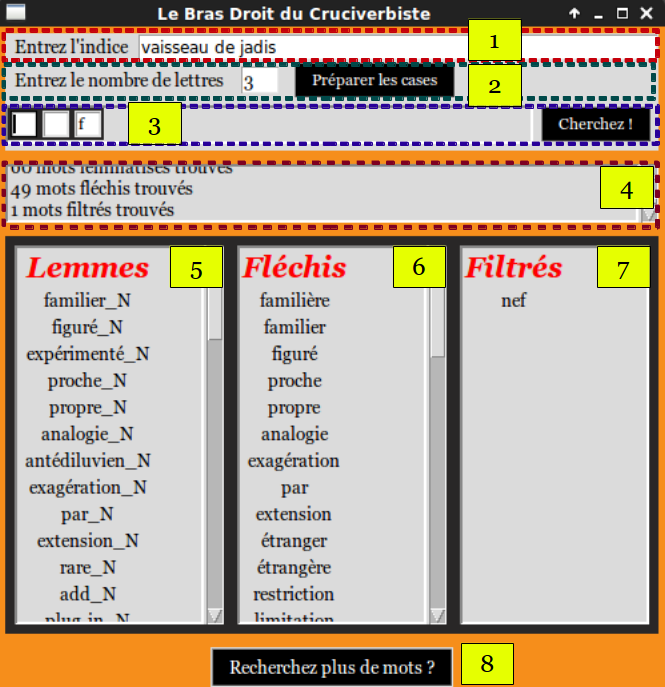
\includegraphics{Images/CrossWordInterface.png}
\end{center}

\begin{enumerate}
    \item{L'indice qui sert à deviner le mot recherché}
    \item{Le nombre de lettres du mot recherché. En cliquant sur \lq{Préparer les cases}\rq, cette contrainte sera enregistrée et les cases générées en 3.}
    \item{Les cases pour entrer les caractères déjà devinés. Cette contrainte sera prise en compte dans le filtrage des mots candidats}
    \item{Le log qui permet de tracer le suivi du programme. Ici seront affichés des avertissements dans le cas où un mot n'est pas reconnu, la/les catégorie(s) syntaxique(s) du mot recherché et le nombre de résultats renvoyés à chaque tour.}
    \item{Les plus proches voisins de l'indice. Au départ les vingt mots les plus proches seront retournés.}
    \item{Les formes fléchies des lemmes renvoyés en 5., qui devraient correspondre aux contraintes flexionnelles imposées par les mots de l'indice, si elles sont reconnues}
    \item{Les candidats filtrés selon les contraint de longueur de mot et de caractères déjà devinés.}
    \item{Si l'utilisateur veut continuer en regardant les vingt prochains plus proches mots, il peut cliquer sur ce bouton pour renvoyer plus de résultats. Ceci peut être utile dans le cas où peu de résultats fléchis ou filtrés sont renvoyés.}
    
\end{enumerate}


\subsection{Evaluation}

\subsection{Améliorations possibles}

\section{Conclusion}
\lstset{literate=
  {á}{{\'a}}1 {é}{{\'e}}1 {í}{{\'i}}1 {ó}{{\'o}}1 {ú}{{\'u}}1
  {Á}{{\'A}}1 {É}{{\'E}}1 {Í}{{\'I}}1 {Ó}{{\'O}}1 {Ú}{{\'U}}1
  {à}{{\`a}}1 {è}{{\`e}}1 {ì}{{\`i}}1 {ò}{{\`o}}1 {ù}{{\`u}}1
  {À}{{\`A}}1 {È}{{\'E}}1 {Ì}{{\`I}}1 {Ò}{{\`O}}1 {Ù}{{\`U}}1
  {ä}{{\"a}}1 {ë}{{\"e}}1 {ï}{{\"i}}1 {ö}{{\"o}}1 {ü}{{\"u}}1
  {Ä}{{\"A}}1 {Ë}{{\"E}}1 {Ï}{{\"I}}1 {Ö}{{\"O}}1 {Ü}{{\"U}}1
  {â}{{\^a}}1 {ê}{{\^e}}1 {î}{{\^i}}1 {ô}{{\^o}}1 {û}{{\^u}}1
  {Â}{{\^A}}1 {Ê}{{\^E}}1 {Î}{{\^I}}1 {Ô}{{\^O}}1 {Û}{{\^U}}1
  {œ}{{\oe}}1 {Œ}{{\OE}}1 {æ}{{\ae}}1 {Æ}{{\AE}}1 {ß}{{\ss}}1
  {ç}{{\c c}}1 {Ç}{{\c C}}1 {ø}{{\o}}1 {å}{{\r a}}1 {Å}{{\r A}}1
  {€}{{\EUR}}1 {£}{{\pounds}}1
}


\appendix
\section{Parametres des poids}\label{App:weights}
%\verbatiminput{../Scripts/Matrices/LITTREMatrix_resources/simplifiedweights.config}

\section{Parametres supplémentaires pour la ponderation des aretes}\label{App:otherparams}
Text of Appendix B is Here

\section{Script de normalisation du Littre}\label{App:normlittre}
%\lstinputlisting[language=Python]{../Scripts/XML/LITTRE_normalisation.py}

\section{Script de normalisation du Wiktionnaire}\label{App:normwiki}
Text of Appendix B is Here

\section{DTD des fichiers XML produits}\label{App:dtddico}
Text of Appendix B is Here

\section{Script utilise pour l'etiquetage syntaxique et la lemmatisation}\label{App:tag}
%\lstinputlisting[language=Python]{../Scripts/XML/tagging_modifs3.py}

\section{Script pour la creation de la matrice}\label{App:creatematrix}
Text of Appendix B is Here


\begin{thebibliography}{10}

\bibitem{wordnet}Princeton University "About WordNet." WordNet. Princeton University. 2010. http://wordnet.princeton.edu \label{bib:wordnet}

\bibitem{WikiXML}WiktionaryX. http://redac.univ-tlse2.fr/lexiques/wiktionaryx.html. Franck Sajous. CLLE-ERSS. \label{bib:wikixml}

\bibitem{LittreXML}Littré, Émile. Dictionnaire de la langue française, Supplément. Paris, L. Hachette, 1878. Electronic version created by François Gannaz. http://www.littre.org \label{bib:littrexml}

\bibitem{MElt}Pascal Denis and Benoît Sagot (2012). Coupling an annotated corpus and a lexicon for state-of-the-art POS tagging. In Language Resources and Evaluation 46:4, pp. 721-736, DOI 10.1007/s10579-012-9193-0\label{bib:melt} 

\bibitem{lefff}Sagot (2010). The Lefff, a freely available and large-coverage morphological and syntactic lexicon for French. In Proceedings of the 7th international conference on Language Resources and Evaluation (LREC 2010), Istanbul, Turkey\label{bib:lefff} 

\end{thebibliography}

\end{document}


